\section{Durchführung}
\label{sec:Durchführung}
Der Versuchaufbau erfolgt gemäß Abbildung \ref{fig:aufbau}.
\begin{figure}
  \centering
  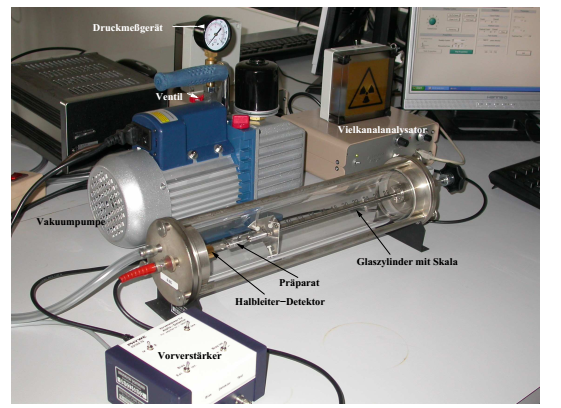
\includegraphics{images/aufbau.png}
  \caption{Versuchsaufbaun entnommen aus der Versuchsanleitung \cite{1}}
  \label{fig:aufbau}
\end{figure}
Dabei wird an die Glasröhre, welche den $\alpha$-Strahler Americium 241 beinhaltet, die Vakuumpumpe sowie ein Vorverstärker mitsamt Vielkanalanalysator angeschlossen.
Letzterer ist an einen Computer angeschlossen auf welchem mit Hilfe der Software Multichannel Analyzer (MCA) die erhaltenen Daten ausgewertet werden.
Zu Beginn des Versuches wird der Glaszylinder evakuiert und der Strahler auf eine Distanz von circa 15 Centimetern geschoben.
Dann wird der Diskriminator so eingestellt, dass mit MCA keine Counts mehr gemessen werden. So werden Störsignale, bei denen es sich nicht um $\alpha$- Strahlung handelt
rausgefiltert. Nun wird der Strahler auf die gewünschte Messdistanz geschoben und zunächst bei evakuiertem Zylinder mit MCA 120 Sekunden lang gemessen. Die Position des
Energiemaximus und die Counts werden dann notiert. Nun wird der Druck hochgeregelt, und bei jedem Druck wird wieder für 120 Sekunden gemessen und die Daten aufgenommen.
Bei erreichen des atmosphärischen Druckes ist die Messung beendet. Dieser Vorgang wird nun für einen zweiten Abstand wiederholt.
Zuletzt wird noch die Statistik des radioaktiven Zerfalls gemessen, indem der Zylinder evakuiert wird, eine Messzeit von zehn Sekunden eingestellt wird und 100 mal gemessen wird.
Bei dieser Messung werden nur die Counts notiert.
